\documentclass[11pt,letterpaper,oneside]{report}

\usepackage[T1]{fontenc}
\usepackage[margin=1in]{geometry}
\usepackage{amsmath}
\usepackage{graphicx}
\usepackage{xcolor}
\usepackage{booktabs}
\usepackage{tabularx}
\usepackage{array}
\usepackage{enumitem}
\usepackage{titlesec}
\usepackage{fancyhdr}
\usepackage[labelsep=period,font=small,labelfont=bf,skip=6pt]{caption}
\usepackage{tikz}
\usetikzlibrary{arrows.meta,positioning,calc,fit,shapes.geometric,shapes.multipart}
\usepackage[hidelinks,pdftitle={Campus Marketplace - UCS503 Software Engineering}]{hyperref}

\definecolor{lg}{gray}{0.88}

% ---------- chapter / section style ----------
\titleformat{\chapter}[display]
  {\raggedleft\bfseries}{\large Chapter \thechapter}{14pt}{\Huge}
\titlespacing*{\chapter}{0pt}{20pt}{28pt}
\titleformat{\section}{\Large\bfseries}{\thesection}{1em}{}
\titleformat{\subsection}{\large\bfseries}{\thesubsection}{1em}{}

% ---------- header / footer ----------
\pagestyle{fancy}
\fancyhf{}
\fancyhead[L]{\small UCS503 -- Software Engineering}
\fancyhead[R]{\small\thepage}
\renewcommand{\headrulewidth}{0.4pt}
\fancypagestyle{plain}{\fancyhf{}\fancyfoot[C]{\small\thepage}\renewcommand{\headrulewidth}{0pt}}

\setlength{\parskip}{4pt}
\setlist{itemsep=2pt,topsep=4pt}

\begin{document}

% ================= COVER =================
\begin{titlepage}
\centering
{\large\bfseries UCS503 -- Software Engineering\par}
\vspace{2.2cm}
{\Huge\bfseries Campus Marketplace\par}
\vspace{0.4cm}
{\small A Verified-Student Platform for Buying, Borrowing, Selling and Lending\\
with ML-Assisted Pricing and Fraud Detection\par}
\vspace{1.6cm}
{\Large\bfseries Submitted by:\par}
\vspace{0.4cm}
\begin{tabular}{ll}
1024031047 & Shweta Agarwal\\
1024031049 & Shrasthi Singh Rathore\\
1024031021 & Raksha Pandey
\end{tabular}\par
\vspace{0.5cm}
{\small Group: 3C73 \quad BE Third Year, CSE\par}
\vspace{1.6cm}
{\Large\bfseries Submitted to:\par}
\vspace{0.4cm}
Dr.\ Johnsy Bansal\par
\vfill
Mid-Semester Evaluation\par
\vspace{0.3cm}
{\bfseries Computer Science and Engineering Department}\par
Thapar Institute of Engineering and Technology, Patiala\par
\end{titlepage}

% ================= FRONT MATTER =================
\pagenumbering{roman}
\setcounter{page}{1}

\chapter*{Abstract}
\addcontentsline{toc}{chapter}{Abstract}
\thispagestyle{plain}

Students on a residential campus constantly need second-hand textbooks, cycles, calculators,
lab equipment and hostel essentials, and just as constantly have such items to pass on.
General-purpose classified platforms are poorly suited to this need: they are open to
anonymous strangers, offer no verification that a seller belongs to the institution, give no
help with fair pricing, and do not support lending with due dates and returns. Campus
Marketplace is a web application that addresses these gaps for a single campus community.

The system lets students with verified college e-mail identities buy, borrow, sell and lend
items. It is built as a React single-page application, an Express.js REST API backed by
MongoDB, and a separate Python FastAPI service that hosts two machine-learning models: a
gradient-boosted quantile regressor that recommends a fair price range, and an Isolation
Forest that scores the fraud risk of every new listing from 22 listing, user and behavioural
features. A combined decision engine publishes low-risk listings, asks the seller for an
extra e-mail verification on medium risk, and holds high-risk listings for an administrator.
Further modules provide e-mail OTP and Google Sign-In verification, duplicate-account
detection, a loan life-cycle with extensions and return confirmation, a payment flow with
server-side signature verification, price-drop alerts, student reports with chat-abuse
reporting, privacy-preserving nearby discovery with encrypted stored locations, a
formula-based trust score with an audit trail, a component-based avatar builder, and an
administrator console for moderation, suspension, analytics and institution settings.

This report documents the requirements, the development methodology, the architecture, and
the implementation of the system, supported by five diagrams (use case, SDLC, sequence,
activity and class). On the held-out test split of the synthetic seed data, the price model
reaches $R^2 = 0.986$, a mean absolute percentage error of 8.7\% and a mean absolute error of
Rs.\ 334, and the fraud model reaches a ROC-AUC of 0.997 with a false-alarm rate below 1\% on
honest users. These figures are reported transparently as baselines, since the models have
not yet been trained on real campus transactions.

\clearpage
\tableofcontents
\clearpage
\listoffigures
\clearpage
\listoftables

% ================= MAIN MATTER =================
\clearpage
\pagenumbering{arabic}
\setcounter{page}{1}

% ---------------- Chapter 1 ----------------
\chapter{Introduction}

\section{Background and Context}
A university campus is a small, dense economy. Every semester, first-year students buy the
same textbooks, drafters and lab coats that graduating students are about to discard; hostel
residents need kettles, mattresses and cycles for a few months only; and short-term needs
such as a scientific calculator for one examination are better served by borrowing than by
purchasing. Today this exchange happens through scattered group chats and notice boards,
which are unsearchable, unstructured and unaccountable.

Public classified websites do not solve the problem. They are open to anyone, so a buyer
cannot tell whether the seller is a genuine fellow student; they provide no guidance on what
a used item is worth; and they have no notion of lending, where an item changes hands for a
limited period and must be returned. A purpose-built, campus-exclusive marketplace can
address each of these shortcomings, and doing so is a good vehicle for applying the full
software engineering life cycle: requirements, design, implementation and evaluation of a
multi-tier, data-driven system.

\subsection{Problem Statement}
Design and implement a web platform in which only verified members of a campus can list
items for sale or for lending, discover items nearby, communicate with each other, complete
purchases or loans with an auditable transaction history, and build a measurable
reputation, while the system itself assists users with fair pricing and protects the
community against fraudulent or duplicated listings.

\section{Project Objectives}
\begin{enumerate}
\item \textbf{Verified access:} restrict the marketplace to users whose college e-mail
identity has been verified (OTP or Google Sign-In), and reject unverified sessions on every
marketplace endpoint.
\item \textbf{Complete trading workflow:} support the four intents buy, borrow, sell and
lend, including a loan life-cycle with due dates, extensions, overdue detection and return
confirmation.
\item \textbf{ML-assisted pricing:} give every seller an explainable fair price range
produced by a trained regression model, with the final price remaining the seller's
decision.
\item \textbf{Fraud screening:} score every new listing for anomalous behaviour, ask the
seller for extra verification on medium risk, and route high-risk listings to an
administrator before they become visible; let students report listings, users and chat
messages.
\item \textbf{Trust and privacy:} compute an explainable trust score for each user with an
audit trail of every change, keep exact coordinates private and encrypted, and reveal meeting
points only after both parties agree.
\item \textbf{Maintainable architecture:} separate the user interface, the business API and
the ML service so that each can be developed, tested and deployed independently, and verify
the API and the models with automated test suites.
\end{enumerate}

\section{Scope and Limitations}
The system targets a single campus whose allowed e-mail domains are configured by the
administrator. Online payment runs in a clearly labelled development mode unless Razorpay
test credentials are supplied. The machine-learning models are trained on synthetic seed
data sets and are therefore a demonstrator of the architecture rather than a
production-grade valuation or fraud engine; both are built to be retrained as real trades
and administrator decisions accumulate. These limitations are discussed again in Chapter~5.

\section{Organisation of the Report}
Chapter~2 lists the stakeholders and the functional and non-functional requirements.
Chapter~3 presents the development methodology and the design through five diagrams.
Chapter~4 describes the implementation and evaluation, and Chapter~5 concludes with
findings, limitations and future work.

% ---------------- Chapter 2 ----------------
\chapter{System Requirements}

\section{Stakeholders and User Roles}
\begin{table}[htbp]
\centering\small
\caption{Stakeholders and their interaction with the system.}
\begin{tabularx}{\textwidth}{@{}lX@{}}
\toprule
\textbf{Role} & \textbf{Description}\\
\midrule
Student & A verified campus member. The same account can act as buyer, borrower, seller or lender, so a single role covers all four intents.\\
Administrator & Reviews held listings in the fraud-alert queue, decides student reports, suspends accounts, manages categories and banned words, and monitors analytics and the audit log.\\
ML service & Internal system actor that returns price recommendations, fraud scores with explanations and model metrics to the API over HTTP.\\
Payment gateway & External actor (Razorpay, or a signed development gateway) that creates orders and confirms payments.\\
Identity provider & Google OAuth 2.0 and an SMTP server used for verification.\\
Image storage & Cloudinary (or local disk in development) for listing photos.\\
\bottomrule
\end{tabularx}
\end{table}

\section{Functional Requirements}
\begin{table}[htbp]
\centering\small
\caption{Functional requirements.}
\begin{tabularx}{\textwidth}{@{}lX@{}}
\toprule
\textbf{ID} & \textbf{Requirement}\\
\midrule
FR1 & A user shall register with a college e-mail, verify it with a one-time password, and log in; Gmail and allowed Google accounts shall use Google Sign-In.\\
FR2 & The system shall reject any marketplace request from an unverified user, and any administrator request from a non-administrator.\\
FR3 & A student shall create, edit, view and remove listings for sale or lending, with category, condition, brand, age, original price, description and images.\\
FR4 & The system shall return a fair-price range, a recommended price, a confidence value and an explanation for a new listing.\\
FR5 & The system shall assign each new listing a fraud-risk score, level (low, medium, high) and explanation; it shall publish low-risk listings, require an e-mailed verification code for medium-risk listings, and hold high-risk listings for review.\\
FR6 & A student shall search and filter listings, keep a watchlist, and receive price-drop alerts with an optional percentage or rupee threshold.\\
FR7 & A student shall chat with a listing owner through stored messages.\\
FR8 & A student shall request to buy or borrow; the owner shall approve or reject, set or change the due date, and approve extensions.\\
FR9 & The system shall track loan status (requested, active, due soon, overdue, return requested, returned, completed) and notify users.\\
FR10 & Sales shall be settled through a payment order whose signature is verified on the server before the sale is marked paid.\\
FR11 & Users shall be able to opt in to nearby discovery; exact coordinates shall never be returned by listing APIs.\\
FR12 & The system shall maintain a trust score from verification, reviews, completed transactions, on-time returns, account age and reports, show its breakdown, and record every change in an audit trail.\\
FR13 & An administrator shall view fraud alerts and approve or reject held listings, confirm or dismiss reports, suspend and restore accounts, view analytics, and manage categories and banned words.\\
FR14 & A student shall report a listing, a user or a received chat message; three open reports shall hide a listing until it is reviewed.\\
FR15 & A student shall edit the profile and build an avatar from components (face, hair, outfit, accessory and colours) without uploading a real photo.\\
FR16 & The system shall detect several accounts created from one device and use it as a fraud signal.\\
\bottomrule
\end{tabularx}
\end{table}

\section{Non-Functional Requirements}
\begin{table}[htbp]
\centering\small
\caption{Non-functional requirements.}
\begin{tabularx}{\textwidth}{@{}lX@{}}
\toprule
\textbf{Attribute} & \textbf{Requirement}\\
\midrule
Security & Passwords hashed with bcrypt; OTPs stored only as salted hashes with expiry, attempt and resend limits; stateless JWT sessions; rate limiting on authentication, OTP and general API traffic; banned-word filtering of listings and messages; suspended accounts blocked on every request.\\
Privacy & Exact latitude and longitude are never exposed and are stored encrypted (AES-256-GCM); approximate distance only, and only for users who opted in; device identifiers stored only as hashes.\\
Availability & The API shall start without an installed MongoDB (in-memory fallback) and shall keep working when the ML service is down.\\
Maintainability & Three independently runnable components with environment-based configuration and a documented REST interface.\\
Usability & Responsive interface; clear labels for development-mode payments and for AI estimates that are not guaranteed market values.\\
Testability & 50 automated API tests and 17 automated model tests covering authentication, listings, location, loans, payments, uploads, the fraud decision engine, reports, administration, alerts and trust score.\\
Accountability & Every trust-score change and every administrator action is written to an append-only audit log with actor and reason.\\
\bottomrule
\end{tabularx}
\end{table}

\section{Hardware and Software Requirements}
\begin{table}[htbp]
\centering\small
\caption{Development and runtime environment.}
\begin{tabularx}{\textwidth}{@{}lX@{}}
\toprule
\textbf{Item} & \textbf{Requirement}\\
\midrule
Client & Any modern browser with JavaScript; Geolocation API for optional nearby discovery.\\
Server & Node.js runtime with npm; MongoDB (local, Atlas, or the bundled in-memory server); Python~3 for the ML service.\\
Libraries & React, React Router, Tailwind CSS, Vite; Express, Mongoose, jsonwebtoken, bcryptjs, nodemailer, multer, Razorpay SDK, Cloudinary SDK, Google Auth Library; FastAPI, scikit-learn, pandas, NumPy, joblib.\\
Hardware & A commodity laptop is sufficient for development and demonstration.\\
\bottomrule
\end{tabularx}
\end{table}

\section{Constraints and Assumptions}
All users hold an e-mail address in an allowed college domain or an allowed Google account.
Trading takes place physically on campus, so the system arranges but does not deliver
exchanges. No map provider key is required; location relies on the browser Geolocation API
and geohashing only.

% ---------------- Chapter 3 ----------------
\chapter{Architecture and Design}

This chapter presents the development methodology and the design of Campus Marketplace. All
diagrams are drawn natively in TikZ and use a monochrome palette: black lines, white fills,
and a light gray for emphasis.

\section{Development Methodology (SDLC)}
The project followed an iterative and incremental life cycle~\cite{larman}. Rather than
building the whole system in one pass, the work was divided into five increments. Each
increment was taken through the same five phases (requirements, design, implementation,
testing, and integration review), and the feedback from the review fed directly into the
requirements of the next increment. Figure~\ref{fig:sdlc} shows the cycle and the
increments delivered. This model suited the project because the user interface existed first
as a prototype on mock data, and the backend, identity, marketplace logic and
machine-learning components were added in successive, independently testable steps.

\begin{figure}[htbp]
\centering
\resizebox{\textwidth}{!}{%
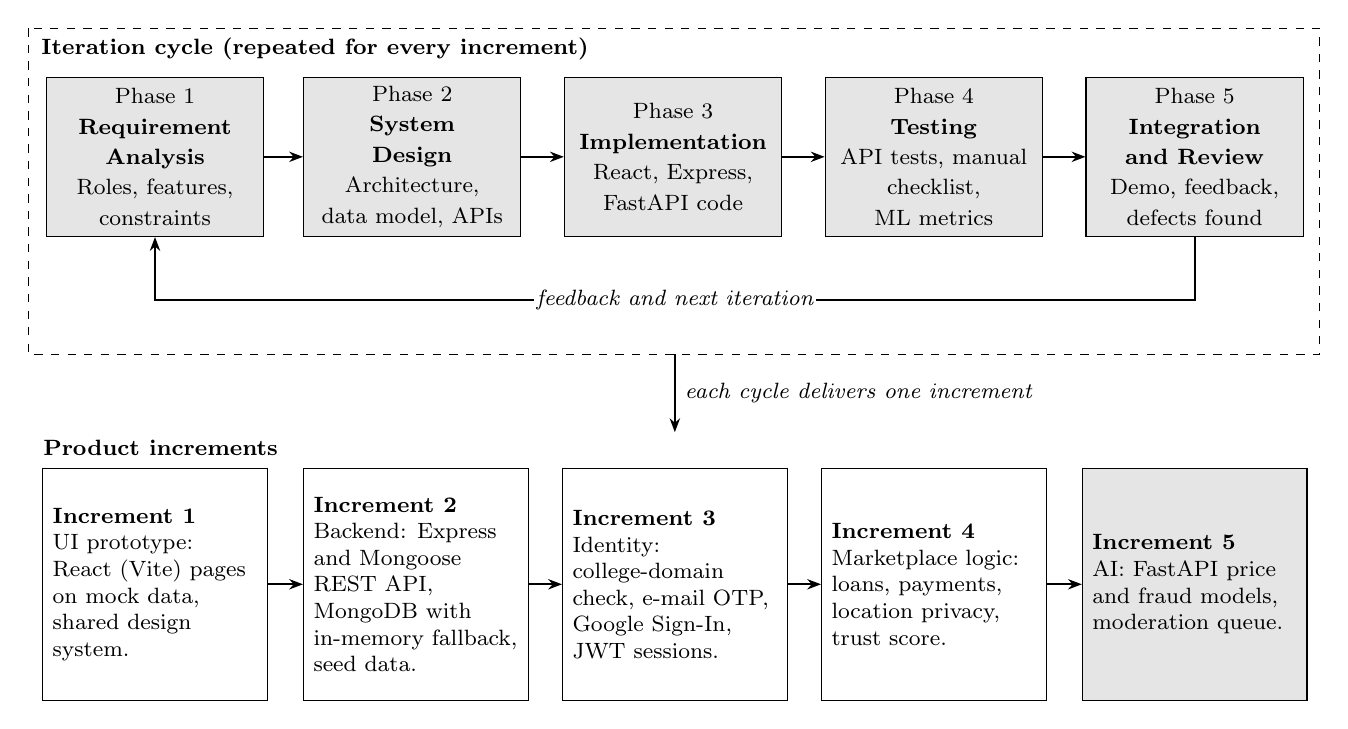
\begin{tikzpicture}[x=0.6545pt,y=-0.6545pt,font=\fontsize{8}{9.6}\selectfont,
  phase/.style={draw,fill=gray!20,execute at begin node=\setlength{\baselineskip}{11pt},minimum width=120*0.6545pt,minimum height=88*0.6545pt,align=center,inner sep=2pt},
  inc/.style={draw,minimum width=124*0.6545pt,minimum height=128*0.6545pt,text width=113*0.6545pt,align=flush left,execute at begin node=\setlength{\baselineskip}{9.6pt},inner sep=3pt},
  arr/.style={-{Stealth[length=5pt]},semithick}]
\draw[dashed] (5,5) rectangle (718,185);
\node[anchor=north west,font=\fontsize{8}{9.6}\selectfont\bfseries,inner sep=0pt] at (12,10) {Iteration cycle (repeated for every increment)};
\node[phase] (p1) at (75,76) {Phase 1\\\textbf{Requirement}\\\textbf{Analysis}\\Roles, features,\\constraints};
\node[phase] (p2) at (217,76) {Phase 2\\\textbf{System}\\\textbf{Design}\\Architecture,\\data model, APIs};
\node[phase] (p3) at (361,76) {Phase 3\\\textbf{Implementation}\\React, Express,\\FastAPI code};
\node[phase] (p4) at (505,76) {Phase 4\\\textbf{Testing}\\API tests, manual\\checklist,\\ML metrics};
\node[phase] (p5) at (649,76) {Phase 5\\\textbf{Integration}\\\textbf{and Review}\\Demo, feedback,\\defects found};
\foreach \a/\b in {p1/p2,p2/p3,p3/p4,p4/p5} \draw[arr] (\a.east) -- (\b.west);
\draw[arr] (p5.south) -- (649,155) -- node[fill=white,font=\fontsize{8}{9.6}\selectfont\itshape,inner sep=1pt] {feedback and next iteration} (75,155) -- (p1.south);
\draw[arr] (362,185) -- node[right,font=\fontsize{8}{9.6}\selectfont\itshape] {each cycle delivers one increment} (362,228);
\node[anchor=north west,font=\fontsize{8}{9.6}\selectfont\bfseries,inner sep=0pt] at (13,232) {Product increments};
\node[inc] (i1) at (75,312) {\textbf{Increment 1}\\UI prototype: React (Vite) pages on mock data, shared design system.};
\node[inc] (i2) at (219,312) {\textbf{Increment 2}\\Backend: Express and Mongoose REST API, MongoDB with in-memory fallback, seed data.};
\node[inc] (i3) at (362,312) {\textbf{Increment 3}\\Identity: college-domain check, e-mail OTP, Google Sign-In, JWT sessions.};
\node[inc] (i4) at (505,312) {\textbf{Increment 4}\\Marketplace logic: loans, payments, location privacy, trust score.};
\node[inc,fill=gray!20] (i5) at (649,312) {\textbf{Increment 5}\\AI: FastAPI price and fraud models, moderation queue.};
\foreach \a/\b in {i1/i2,i2/i3,i3/i4,i4/i5} \draw[arr] (\a.east) -- (\b.west);
\end{tikzpicture}%
}
\caption{SDLC diagram: iterative and incremental model used for Campus Marketplace.}
\label{fig:sdlc}
\end{figure}

\section{Use Case Model}
Figure~\ref{fig:usecase} shows the use cases inside the system boundary. A single Student
actor covers buyer, borrower, seller and lender because the same account performs all four
roles. The administrator moderates held listings (and, in the final system, also decides
student reports, suspends accounts and manages institution settings); the ML service and the
payment gateway are secondary actors that the system calls. Price prediction and fraud scoring \emph{extends}
listing creation, and making a payment \emph{includes} signature verification.

\begin{figure}[htbp]
\centering
\begin{tikzpicture}[
  uc/.style={draw,ellipse,minimum width=3.5cm,minimum height=0.95cm,align=center,font=\scriptsize,inner sep=1pt},
  ucg/.style={uc,fill=lg},
  assoc/.style={thick},
  rel/.style={-{Stealth[length=5pt]},dashed},
  rl/.style={font=\scriptsize,inner sep=1.5pt,fill=white}
]
\tikzset{actor/.pic={
  \draw (0,0.55) circle (0.17);
  \draw (0,0.38) -- (0,-0.15) (-0.28,0.22) -- (0.28,0.22) (0,-0.15) -- (-0.22,-0.65) (0,-0.15) -- (0.22,-0.65);
}}
% system boundary
\draw (1.8,1.0) rectangle (12.5,-11.2);
\node[font=\small\bfseries] at (7.15,0.65) {Campus Marketplace System};
% student use cases
\node[uc] (u1) at (4.3,-0.5)  {Register and Verify\\College E-mail\\(OTP / Google Sign-In)};
\node[uc] (u2) at (4.3,-1.85) {Browse, Search\\and Filter Listings};
\node[uc] (u3) at (4.3,-3.1)  {Manage Watchlist\\and Notifications};
\node[uc] (u4) at (4.3,-4.35) {Create Listing\\(Sell / Lend)};
\node[uc] (u5) at (4.3,-5.6)  {Chat with\\Listing Owner};
\node[uc] (u6) at (4.3,-6.85) {Request to\\Buy / Borrow};
\node[uc] (u7) at (4.3,-8.1)  {Make Payment};
\node[uc] (u8) at (4.3,-9.3)  {Approve, Extend\\and Return Loans};
\node[uc] (u9) at (4.3,-10.5) {Review and Rate Users};
% admin / system use cases
\node[ucg] (a1) at (10.2,-0.5)  {Review Fraud Alerts};
\node[ucg] (a2) at (10.2,-1.85) {Approve / Reject\\Held Listing};
\node[ucg] (m1) at (10.2,-3.4)  {Predict Fair\\Price Range};
\node[ucg] (m2) at (10.2,-5.3)  {Score Listing\\Fraud Risk};
\node[ucg] (p1) at (10.2,-8.1)  {Verify Payment\\Signature};
% actors
\pic at (0.5,-5.2) {actor};
\node[font=\scriptsize,fill=white,inner sep=1pt] at (0.5,-6.15) {Student};
\pic at (14.0,-1.1) {actor};
\node[font=\scriptsize,align=center] at (14.0,-2.0) {Administrator};
\pic at (14.0,-4.3) {actor};
\node[font=\scriptsize,align=center] at (14.0,-5.2) {ML service\\(FastAPI)};
\pic at (14.0,-8.1) {actor};
\node[font=\scriptsize,align=center] at (14.0,-9.0) {Payment\\Gateway\\(Razorpay)};
% associations
\foreach \n in {u1,u2,u3,u4,u5,u6,u7,u8,u9}
  \draw[assoc] (0.5,-5.2) -- (\n.west);
\draw[assoc] (14.0,-1.1) -- (a1.east);
\draw[assoc] (14.0,-1.1) -- (a2.east);
\draw[assoc] (14.0,-4.3) -- (m1.east);
\draw[assoc] (14.0,-4.3) -- (m2.east);
\draw[assoc] (14.0,-8.1) -- (p1.east);
% extends / includes
\draw[rel] (m1.west) -- (u4.east) node[pos=0.5,above,sloped,font=\scriptsize,inner sep=1pt]{\guillemotleft extends\guillemotright};
\draw[rel] (m2.west) -- (u4.east) node[pos=0.5,above,sloped,font=\scriptsize,inner sep=1pt]{\guillemotleft extends\guillemotright};
\draw[rel] (u7.east) -- (p1.west) node[midway,rl]{\guillemotleft includes\guillemotright};
\end{tikzpicture}
\caption{Use case diagram of Campus Marketplace.}
\label{fig:usecase}
\end{figure}

\section{Sequence Model}
The system is organised as three independently runnable tiers: a React single-page
application that talks only to the REST API through a central client module, an Express.js
API that applies CORS, rate limiting and JWT authentication before requests reach the route
modules and business services, and a separate FastAPI service that hosts the price and fraud
models. Persistent data lives in MongoDB, and identity and payment providers are external
services. Keeping the ML stack in its own service means it can be trained, replaced or
restarted without touching the API, and the API degrades gracefully when that service is
unreachable.

Figure~\ref{fig:sequence} shows how these parts interact over time when a seller publishes
a listing. The seller submits the details through the interface, which sends a request to the
API. The API asks the ML service for a fair-price range, then for a fraud-risk score (the
recommended price is passed in as one of the fraud features), saves the listing in MongoDB
with the resulting status, and returns the result and its explanation to the interface for
display.

\begin{figure}[htbp]
\centering
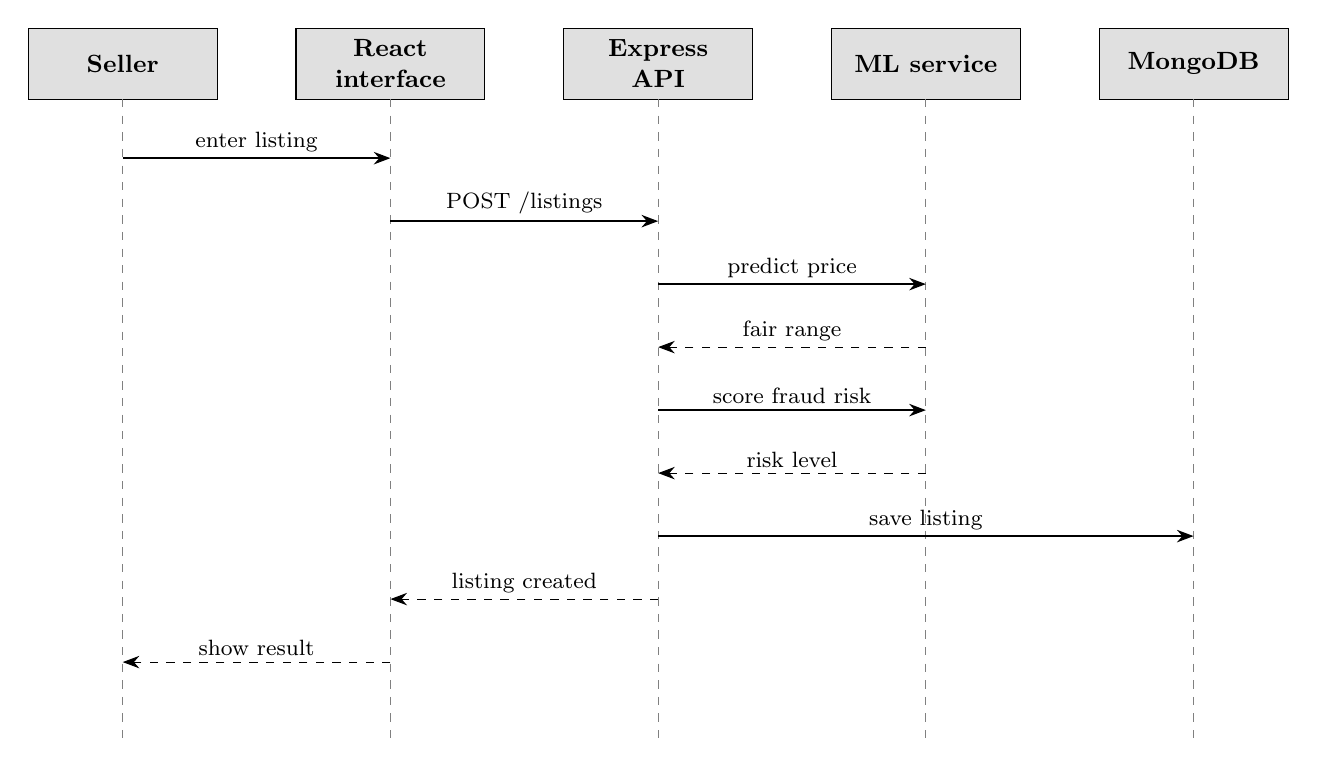
\begin{tikzpicture}[
  part/.style={draw,fill=lg,minimum width=2.4cm,minimum height=0.9cm,align=center,font=\small\bfseries},
  life/.style={dashed,gray},
  msg/.style={-{Stealth[length=6pt]},thick},
  ret/.style={-{Stealth[length=6pt]},dashed},
  lbl/.style={above,inner sep=2pt,font=\footnotesize}
]
\node[part] (s)   at (0,0)    {Seller};
\node[part] (ui)  at (3.4,0)  {React\\interface};
\node[part] (api) at (6.8,0)  {Express\\API};
\node[part] (ml)  at (10.2,0) {ML service};
\node[part] (db)  at (13.6,0) {MongoDB};
\foreach \x in {0,3.4,6.8,10.2,13.6}
  \draw[life] (\x,-0.45) -- (\x,-8.6);
\draw[msg] (0,-1.2)    -- (3.4,-1.2)   node[midway,lbl]{enter listing};
\draw[msg] (3.4,-2.0)  -- (6.8,-2.0)   node[midway,lbl]{POST /listings};
\draw[msg] (6.8,-2.8)  -- (10.2,-2.8)  node[midway,lbl]{predict price};
\draw[ret] (10.2,-3.6) -- (6.8,-3.6)   node[midway,lbl]{fair range};
\draw[msg] (6.8,-4.4)  -- (10.2,-4.4)  node[midway,lbl]{score fraud risk};
\draw[ret] (10.2,-5.2) -- (6.8,-5.2)   node[midway,lbl]{risk level};
\draw[msg] (6.8,-6.0)  -- (13.6,-6.0)  node[midway,lbl]{save listing};
\draw[ret] (6.8,-6.8)  -- (3.4,-6.8)   node[midway,lbl]{listing created};
\draw[ret] (3.4,-7.6)  -- (0,-7.6)     node[midway,lbl]{show result};
\end{tikzpicture}
\caption{Sequence diagram: publishing a listing with price recommendation and fraud screening.}
\label{fig:sequence}
\end{figure}

\section{Activity Model}
Figure~\ref{fig:activity} traces the end-to-end flow from sign-in to a completed transaction.
A user first proves a verified college identity. A seller then enters listing details, the ML
service returns a fair-price range, and after the seller fixes an asking price the system
computes a fraud-risk score; a high-risk listing is held and goes live only if an
administrator approves it. A medium-risk listing (not drawn separately in the figure) waits
for a one-time code e-mailed to the seller before it becomes active, and a low-risk listing
is published at once. A buyer later requests the item; if the owner approves, a sale
proceeds through payment-signature verification, while a loan proceeds through agreement on a
meeting point and due date and ends with a lender-confirmed return. Rejections terminate the
flow at activity final nodes.

\begin{figure}[p]
\centering
\resizebox{!}{0.78\textheight}{%
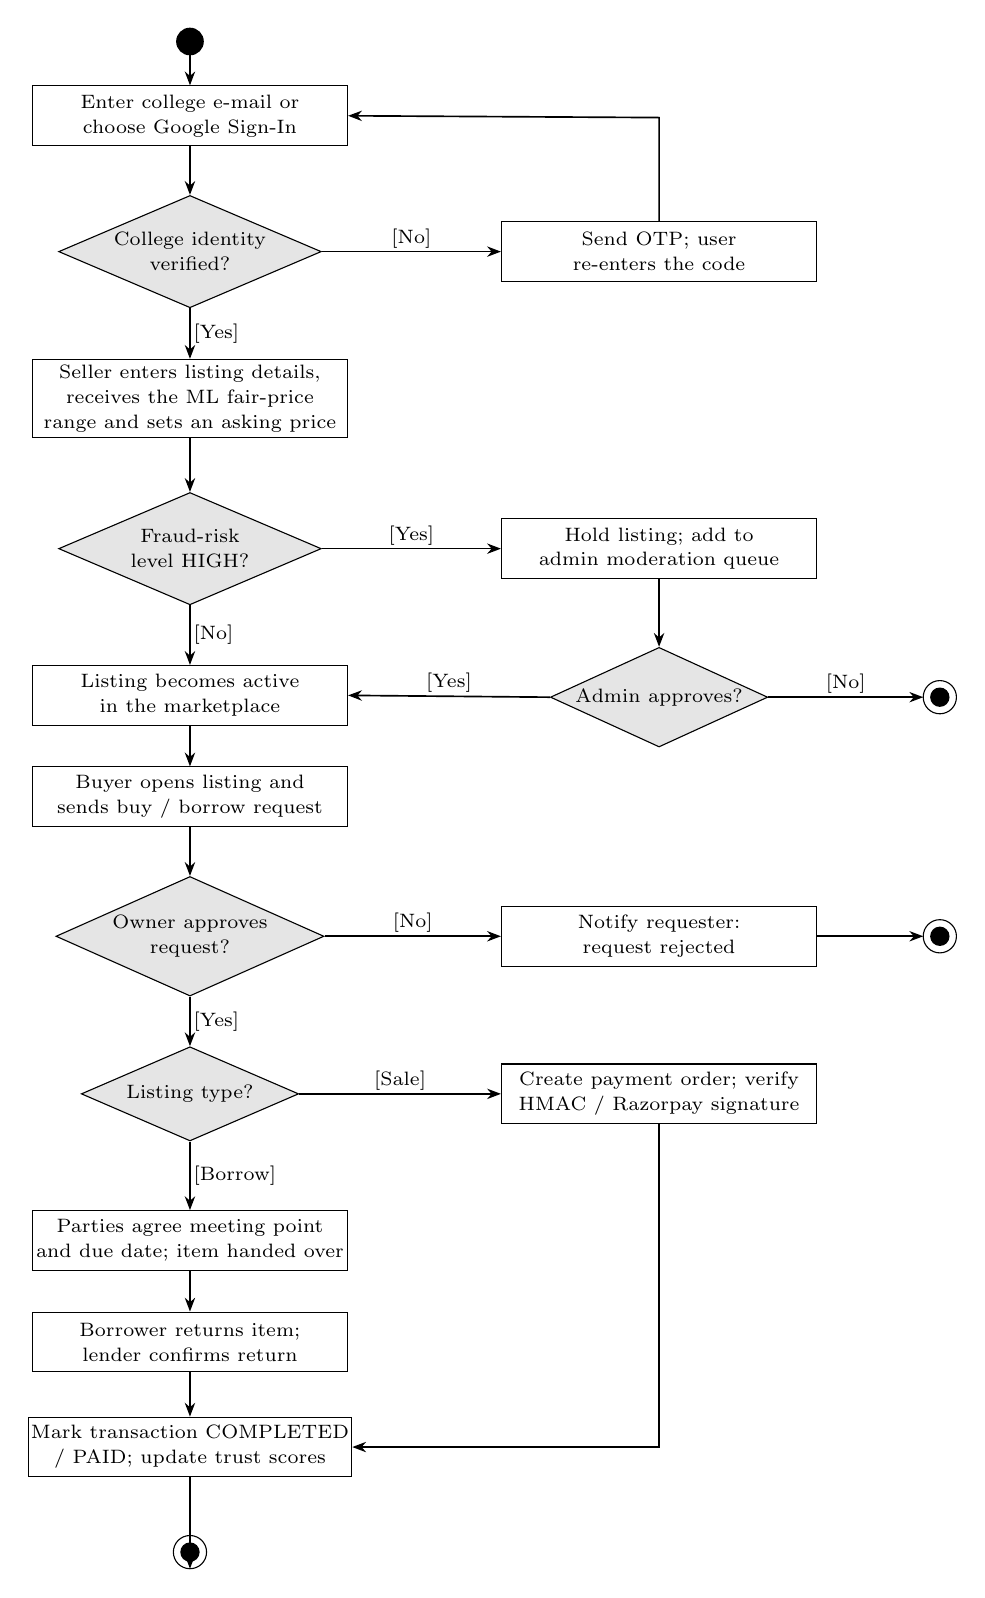
\begin{tikzpicture}[x=0.6545pt,y=-0.6545pt,font=\fontsize{7.5}{9}\selectfont,
  act/.style={draw,minimum width=174*0.6545pt,minimum height=33*0.6545pt,align=center,inner sep=1pt},
  dec/.style={draw,diamond,fill=gray!20,aspect=2.3,align=center,inner sep=0.5pt},
  arr/.style={-{Stealth[length=5pt]},semithick},
  lab/.style={font=\fontsize{7.5}{9}\selectfont,inner sep=1pt}]

\fill (93,13) circle (5pt);
\node[act] (a1) at (93,54) {Enter college e-mail or\\choose Google Sign-In};
\node[dec,minimum width=145*0.6545pt,minimum height=62*0.6545pt] (d1) at (93,129) {College identity\\verified?};
\node[act] (b1) at (352,129) {Send OTP; user\\re-enters the code};
\node[act,minimum height=43*0.6545pt] (a2) at (93,210) {Seller enters listing details,\\receives the ML fair-price\\range and sets an asking price};
\node[dec,minimum width=145*0.6545pt,minimum height=62*0.6545pt] (d2) at (93,293) {Fraud-risk\\level HIGH?};
\node[act] (b2) at (352,293) {Hold listing; add to\\admin moderation queue};
\node[dec,minimum width=120*0.6545pt,minimum height=55*0.6545pt] (d3) at (352,375) {Admin approves?};
\node[act] (a3) at (93,374) {Listing becomes active\\in the marketplace};
\node[act] (a4) at (93,430) {Buyer opens listing and\\sends buy / borrow request};
\node[dec,minimum width=148*0.6545pt,minimum height=66*0.6545pt] (d4) at (93,507) {Owner approves\\request?};
\node[act] (b3) at (352,507) {Notify requester:\\request rejected};
\node[dec,minimum width=120*0.6545pt,minimum height=52*0.6545pt] (d5) at (93,594) {Listing type?};
\node[act] (b4) at (352,594) {Create payment order; verify\\HMAC / Razorpay signature};
\node[act] (a5) at (93,675) {Parties agree meeting point\\and due date; item handed over};
\node[act] (a6) at (93,731) {Borrower returns item;\\lender confirms return};
\node[act] (a7) at (93,789) {Mark transaction COMPLETED\\/ PAID; update trust scores};
\coordinate (e1) at (507,375); \coordinate (e2) at (507,507); \coordinate (e3) at (93,847);
\foreach \e in {e1,e2,e3} {\draw (\e) circle (6pt); \fill (\e) circle (3.5pt);}
\draw[arr] (93,20) -- (a1.north);
\draw[arr] (a1) -- (d1);
\draw[arr] (d1.east) -- node[lab,above] {[No]} (b1.west);
\draw[arr] (b1.north) -- (352,55) -- (a1.east);
\draw[arr] (d1.south) -- node[lab,right] {[Yes]} (a2.north);
\draw[arr] (a2) -- (d2);
\draw[arr] (d2.east) -- node[lab,above] {[Yes]} (b2.west);
\draw[arr] (b2) -- (d3);
\draw[arr] (d2.south) -- node[lab,right] {[No]} (a3.north);
\draw[arr] (d3.west) -- node[lab,above] {[Yes]} (a3.east);
\draw[arr] (d3.east) -- node[lab,above] {[No]} ($(e1)+(-6pt,0)$);
\draw[arr] (a3) -- (a4);
\draw[arr] (a4) -- (d4);
\draw[arr] (d4.east) -- node[lab,above] {[No]} (b3.west);
\draw[arr] (b3.east) -- ($(e2)+(-6pt,0)$);
\draw[arr] (d4.south) -- node[lab,right] {[Yes]} (d5.north);
\draw[arr] (d5.east) -- node[lab,above] {[Sale]} (b4.west);
\draw[arr] (d5.south) -- node[lab,right] {[Borrow]} (a5.north);
\draw[arr] (a5) -- (a6);
\draw[arr] (a6) -- (a7);
\draw[arr] (b4.south) -- (352,789) -- (a7.east);
\draw[arr] (a7.south) -- ($(e3)+(0,-6pt)$);
\end{tikzpicture}%
}
\caption{Activity diagram: sign-in, listing, moderation and transaction flow.}
\label{fig:activity}
\end{figure}

\section{Class Model}
Figure~\ref{fig:class} shows the principal persistent classes. Each class maps to a Mongoose
schema and a MongoDB collection; the attribute lists are abbreviated to the fields central to
the design. User is the hub: it owns listings, takes part in transactions, sends and receives
messages, and receives reviews. A Listing is the subject of transactions and may be screened
in the Moderation queue. A Transaction may be settled by one Payment. Types such as Number
and ObjectId follow the Mongoose schema types. Supporting collections that are not drawn
(Notification, Watchlist, Upload, FraudReport, AuditLog and Settings) reference User and
Listing in the same way.

\begin{figure}[p]
\centering
\resizebox{\textwidth}{!}{%
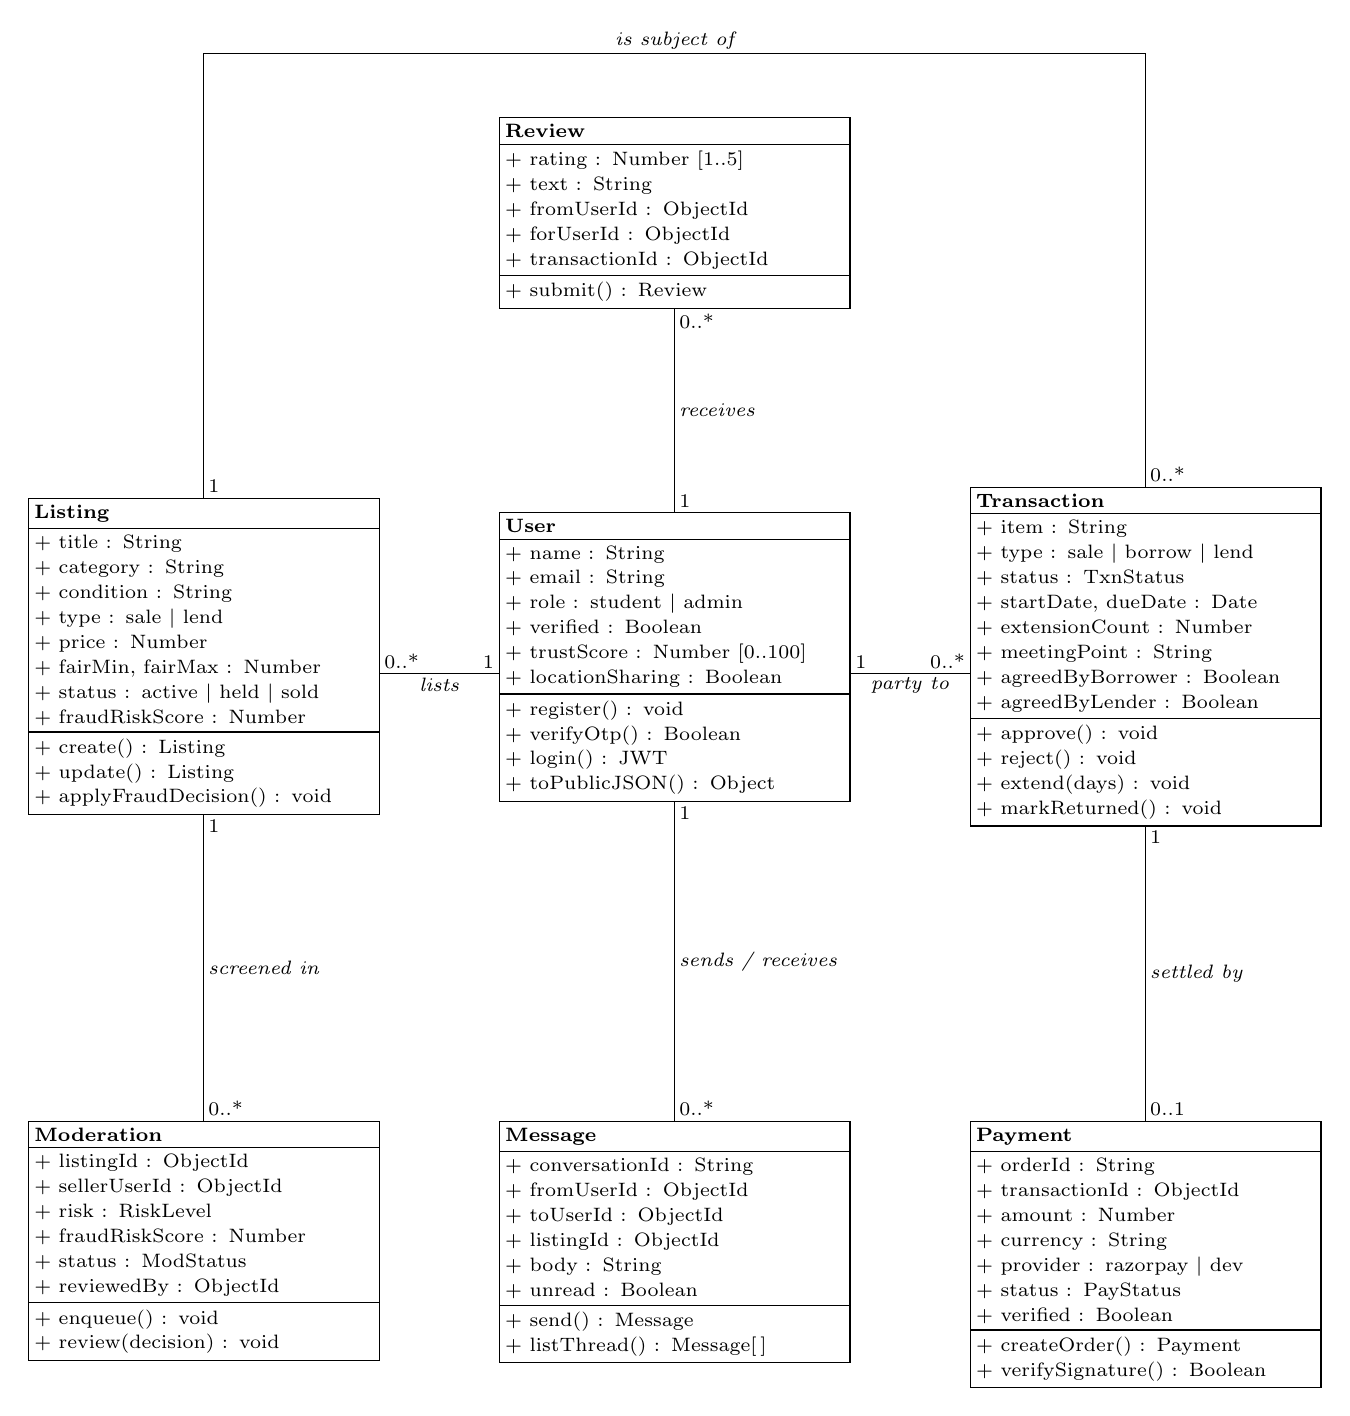
\begin{tikzpicture}[x=0.6545pt,y=-0.6545pt,font=\fontsize{7.5}{9}\selectfont,
  cls/.style={draw,rectangle split,rectangle split parts=3,text width=187*0.6545pt,align=left,inner sep=2.2pt,anchor=north west},
  mult/.style={font=\fontsize{7.5}{9}\selectfont,inner sep=1.5pt},
  role/.style={font=\fontsize{7.5}{9}\selectfont\itshape,inner sep=1.5pt}]
\node[cls] (rev) at (265,55) {\textbf{Review}\nodepart{two}+ rating : Number [1..5]\\+ text : String\\+ fromUserId : ObjectId\\+ forUserId : ObjectId\\+ transactionId : ObjectId\nodepart{three}+ submit() : Review};
\node[cls] (lis) at (5,265) {\textbf{Listing}\nodepart{two}+ title : String\\+ category : String\\+ condition : String\\+ type : sale $|$ lend\\+ price : Number\\+ fairMin, fairMax : Number\\+ status : active $|$ held $|$ sold\\+ fraudRiskScore : Number\nodepart{three}+ create() : Listing\\+ update() : Listing\\+ applyFraudDecision() : void};
\node[cls] (usr) at (265,273) {\textbf{User}\nodepart{two}+ name : String\\+ email : String\\+ role : student $|$ admin\\+ verified : Boolean\\+ trustScore : Number [0..100]\\+ locationSharing : Boolean\nodepart{three}+ register() : void\\+ verifyOtp() : Boolean\\+ login() : JWT\\+ toPublicJSON() : Object};
\node[cls] (txn) at (525,259) {\textbf{Transaction}\nodepart{two}+ item : String\\+ type : sale $|$ borrow $|$ lend\\+ status : TxnStatus\\+ startDate, dueDate : Date\\+ extensionCount : Number\\+ meetingPoint : String\\+ agreedByBorrower : Boolean\\+ agreedByLender : Boolean\nodepart{three}+ approve() : void\\+ reject() : void\\+ extend(days) : void\\+ markReturned() : void};
\node[cls] (mod) at (5,609) {\textbf{Moderation}\nodepart{two}+ listingId : ObjectId\\+ sellerUserId : ObjectId\\+ risk : RiskLevel\\+ fraudRiskScore : Number\\+ status : ModStatus\\+ reviewedBy : ObjectId\nodepart{three}+ enqueue() : void\\+ review(decision) : void};
\node[cls] (msg) at (265,609) {\textbf{Message}\nodepart{two}+ conversationId : String\\+ fromUserId : ObjectId\\+ toUserId : ObjectId\\+ listingId : ObjectId\\+ body : String\\+ unread : Boolean\nodepart{three}+ send() : Message\\+ listThread() : Message[\,]};
\node[cls] (pay) at (525,609) {\textbf{Payment}\nodepart{two}+ orderId : String\\+ transactionId : ObjectId\\+ amount : Number\\+ currency : String\\+ provider : razorpay $|$ dev\\+ status : PayStatus\\+ verified : Boolean\nodepart{three}+ createOrder() : Payment\\+ verifySignature() : Boolean};
% Review -- User
\draw (rev.south) -- (usr.north);
\node[mult,anchor=north west] at (rev.south) {0..*}; \node[mult,anchor=south west] at (usr.north) {1};
\node[role,anchor=west] at ($(rev.south)!0.5!(usr.north)$) {receives};
% Listing -- User
\draw (lis.east |- 0,362) -- (usr.west |- 0,362);
\node[mult,anchor=south west] at (lis.east |- 0,362) {0..*}; \node[mult,anchor=south east] at (usr.west |- 0,362) {1};
\node[role,anchor=north] at ($(lis.east |- 0,362)!0.5!(usr.west |- 0,362)$) {lists};
% User -- Transaction
\draw (usr.east |- 0,362) -- (txn.west |- 0,362);
\node[mult,anchor=south west] at (usr.east |- 0,362) {1}; \node[mult,anchor=south east] at (txn.west |- 0,362) {0..*};
\node[role,anchor=north] at ($(usr.east |- 0,362)!0.5!(txn.west |- 0,362)$) {party to};
% Listing -- Moderation
\draw (lis.south) -- (mod.north);
\node[mult,anchor=north west] at (lis.south) {1}; \node[mult,anchor=south west] at (mod.north) {0..*};
\node[role,anchor=west] at ($(lis.south)!0.5!(mod.north)$) {screened in};
% User -- Message
\draw (usr.south) -- (msg.north);
\node[mult,anchor=north west] at (usr.south) {1}; \node[mult,anchor=south west] at (msg.north) {0..*};
\node[role,anchor=west] at ($(usr.south)!0.5!(msg.north)$) {sends / receives};
% Transaction -- Payment
\draw (txn.south) -- (pay.north);
\node[mult,anchor=north west] at (txn.south) {1}; \node[mult,anchor=south west] at (pay.north) {0..1};
\node[role,anchor=west] at ($(txn.south)!0.5!(pay.north)$) {settled by};
% Listing -- Transaction (is subject of)
\draw (lis.north) -- (lis.north |- 0,20) -- (txn.north |- 0,20) -- (txn.north);
\node[mult,anchor=south west] at (lis.north) {1}; \node[mult,anchor=south west] at (txn.north) {0..*};
\node[role,anchor=south] at ($(lis.north |- 0,20)!0.5!(txn.north |- 0,20)$) {is subject of};
\end{tikzpicture}%
}
\caption{Class diagram of the persistent domain model.}
\label{fig:class}
\end{figure}

% ---------------- Chapter 4 ----------------
\chapter{Implementation}

\section{Technology Stack}
\begin{table}[htbp]
\centering\small
\caption{Technology stack by layer.}
\begin{tabularx}{\textwidth}{@{}l>{\raggedright\arraybackslash}p{4.2cm}X@{}}
\toprule
\textbf{Layer} & \textbf{Technology} & \textbf{Purpose}\\
\midrule
Frontend & React 19, React Router 7, Vite, Tailwind CSS~\cite{react} & Single-page UI, protected routes, filters, favourites, dashboards.\\
API & Node.js, Express 4~\cite{express}, Mongoose & REST endpoints, validation, business rules.\\
Database & MongoDB~\cite{mongo} & Persistence for users, listings, loans, messages, payments and reviews.\\
Security & jsonwebtoken, bcryptjs, express-rate-limit & Sessions~\cite{jwt}, password hashing, throttling.\\
Identity & Google Auth Library, nodemailer & OAuth 2.0 sign-in~\cite{oauth} and OTP e-mail.\\
Payments & Razorpay SDK, HMAC-SHA256~\cite{hmac} & Order creation, signature verification, webhooks and refunds.\\
Storage & Cloudinary, multer & Validated photo upload, resizing and clean-up.\\
ML service & Python, FastAPI~\cite{fastapi}, scikit-learn~\cite{sklearn}, pandas, joblib & Quantile price regression and fraud anomaly scoring.\\
Quality & oxlint, Node test runner, Python unittest & Static analysis, API tests and model tests.\\
\bottomrule
\end{tabularx}
\end{table}

The repository is organised so that each tier can be run on its own: \texttt{src/} holds the
React pages and components; \texttt{server/models}, \texttt{server/routes},
\texttt{server/middleware} and \texttt{server/utils} hold the Mongoose schemas, REST routers,
authentication and rate-limit middleware, and business services; \texttt{server/seed.js}
creates demonstration data; and \texttt{ml-service/} contains the FastAPI application, the
training scripts, the seed data set and the serialised models.

\section{Frontend}
The interface is a React single-page application with ten routes: sign-in and the Google
callback, a dashboard, Buy/Borrow, Sell/Lend, My Listings, Messages, Transactions,
Notifications, Profile and the administrator console. A Protected wrapper redirects
unauthenticated visitors to the sign-in page. All network access goes through one module,
\texttt{src/api.js}, which attaches the JWT to each request. During development Vite proxies
\texttt{/api} to the Express server, which removed the cross-origin problems that had
initially appeared between the two ports.

Listings originally referenced Lucide icon components, which cannot be stored in a database.
The schema therefore stores a string \texttt{iconKey} and the client maps it back to a
component when a listing is rendered (\texttt{hydrateListing}).

The final interface adds the components that expose the AI and trust features to users: a
price-insight panel, a verification panel in which a seller enters the e-mailed code for a
medium-risk listing, a report button on listings and received chat messages, a price-drop
alert control on the listing page, a trust-score breakdown with its change history on the
profile, an SVG avatar builder, and an administrator console with tabs for fraud alerts,
reports, users, analytics, settings, model metrics and the audit log. The categories offered
to sellers are loaded from the server so that administrators can enable, disable or add
them.

\section{Backend REST API}
The Express application applies CORS, JSON parsing with a body-size limit, a global rate
limiter and an optional-authentication middleware before mounting the routers summarised in
Table~\ref{tab:api}. Every marketplace route is wrapped by \texttt{requireAuth} and
\texttt{requireVerified}; administrator routes additionally use \texttt{requireAdmin}. A
health endpoint reports the database state, the payment mode and the ML service address.

\begin{table}[htbp]
\centering\small
\caption{REST API modules (all under \texttt{/api}).}
\label{tab:api}
\begin{tabularx}{\textwidth}{@{}l l X@{}}
\toprule
\textbf{Module} & \textbf{Prefix} & \textbf{Operations}\\
\midrule
Auth & \texttt{/auth} & register, resend-otp, verify, login, logout, me, google, google/start, google/callback\\
Listings & \texttt{/listings} & search and list, mine, read, create, update, delete, verify, resend verification code, location\\
Transactions & \texttt{/transactions} & request, approve, reject, due-date, return, extend, meeting\\
Payments & \texttt{/payments} & create-order, verify, dev-complete, read\\
Messages & \texttt{/messages} & list conversations, read thread, send\\
Watchlist & \texttt{/watchlist} & list, add, update alert threshold, remove\\
Reports & \texttt{/reports} & report listing, user or message; my reports\\
Uploads & \texttt{/uploads} & status, upload images, delete image\\
Notifications & \texttt{/notifications} & list, mark as read\\
Location & \texttt{/location} & preferences, update position, nearby\\
Users, reviews & \texttt{/users} & profile, update profile and avatar, avatar options, trust-score, reviews\\
AI & \texttt{/ai} & price-predict, fraud-score\\
Admin & \texttt{/admin} & fraud-alerts, review of a held listing, reports and decisions, users and suspension, analytics, settings, audit log, fraud-model metrics\\
\bottomrule
\end{tabularx}
\end{table}

\section{Authentication and Verified Access}
Registration accepts only addresses in the configured college domains. The server generates
a one-time password, stores only a salted hash of it together with an expiry time, an
attempt counter and a resend counter, and delivers it by SMTP (or returns it in the response
when a development flag is set). Passwords are hashed with bcrypt. Verification failures,
expired codes and rapid resends are limited by dedicated rate limiters.

Users with a Google account follow the OAuth 2.0 authorization-code flow~\cite{oauth}: the
API redirects to Google's account picker, exchanges the returned code, checks that the e-mail
address is verified by Google and belongs to an allowed domain, and then issues the same
JWT~\cite{jwt} that password login produces. Because the token carries only the user
identity, the API remains stateless; the verified flag and role are re-read from the database
on every request, so revoking verification or suspending an account takes effect
immediately.

To detect duplicate accounts, the browser sends a random per-device identifier with every
request. The server stores only a peppered SHA-256 hash of it on the user, refuses new
sign-ups once a configurable number of accounts already exist on one device, and reports the
number of other accounts sharing a device as the \emph{linked accounts} fraud feature.

\section{Listings, Fair-Price Assistance and Fraud Screening}

\subsection{Creating a listing}
When a seller publishes a listing, the API validates the input, rejects disabled categories
and banned words, requests a price recommendation, stores the recommended range on the
listing, and then assesses fraud risk. If the ML service cannot be reached, the listing is
still created: the price falls back to the formula of Table~\ref{tab:cond} and the fraud
check to a rule-based score with the same thresholds, and both are labelled as fallbacks in
the interface. When an active listing is later edited, it is screened again so that a
listing cannot be turned into a scam after it has been published.

\subsection{Price recommendation}
The price model predicts the scale-free target $\log(\text{price}/\text{original price})$, so
that a Rs.\ 900 calculator and a Rs.\ 40{,}000 laptop are learned on the same scale. Its 28
encoded features are the logarithm of the original price, the age in months, the condition,
the demand, a brand tier, sale or lend with the lending unit, the category, and an item class
inferred from the title (phone, laptop, textbook, cycle and others). Three histogram
gradient-boosting regressors~\cite{friedman} are trained with the quantile loss at the 10th,
50th and 90th percentiles: the median gives the recommended price and the outer quantiles the
fair range. Monotone constraints guarantee that an older item is never priced higher and a
better condition never lower. Because raw quantile models tend to under-cover, the band is
widened by conformalised quantile regression~\cite{romano} on a held-out calibration split
until about 80\% of true prices fall inside it. The reported confidence decreases as the
band widens relative to the price. The condition factors of Table~\ref{tab:cond} are now
used only by the fallback formula when the ML service is offline. The seller can ignore the
suggestion; the asking price is always the seller's choice.

\begin{table}[htbp]
\centering\small
\caption{Condition factors used by the fair-price formula.}
\label{tab:cond}
\begin{tabular}{@{}lcccc@{}}
\toprule
\textbf{Condition} & New & Like New & Good & Fair\\
\midrule
\textbf{Factor} & 0.92 & 0.78 & 0.62 & 0.45\\
\bottomrule
\end{tabular}
\end{table}

\subsection{Fraud scoring}
For each new listing the API assembles 22 features at three levels (Table~\ref{tab:fraudfeat}).
Each feature is oriented so that a larger value means more risk and is clipped on its safe
side, so that unusually \emph{good} behaviour (a four-year-old account, a long description, a
price above the fair range) can never make a listing look anomalous. The FastAPI service
evaluates the vector with an Isolation Forest~\cite{liu} of 400 trees, which isolates
anomalies with few random splits and needs no fraud labels. The raw anomaly value is
calibrated to a fraud risk score between 0 and 1 by interpolating between percentiles of the
training scores. As a guardrail, two or more independent rule-based red flags always raise the
score to at least the medium threshold.

\begin{table}[htbp]
\centering\small
\caption{Fraud-model features by level.}
\label{tab:fraudfeat}
\begin{tabularx}{\textwidth}{@{}lX@{}}
\toprule
\textbf{Level} & \textbf{Features}\\
\midrule
Listing & Price below the AI fair price; price below the median of comparable campus listings; discount on an expensive item; price; short title; short description; same title re-posted; copied description; no photos; photos already used by another seller (SHA-256 of the uploaded file); phone, UPI or ``pay outside the app'' text; urgency words.\\
User & New account; unverified e-mail; other accounts on the same device; confirmed reports; open reports; low trust score.\\
Behavioural & Listings in the last hour; listings in the last 24 hours; outgoing messages in the last hour; transactions in the last 24 hours.\\
\bottomrule
\end{tabularx}
\end{table}

A combined decision engine maps the score to an action (Table~\ref{tab:decision}). A low price
on its own is only one of the 22 inputs, so a genuine bargain from an established seller stays
low risk. Every score is returned with up to three human-readable reasons, computed by
occlusion: each feature in turn is reset to its typical value and the drop in risk is
measured. The reasons are shown to the seller and in the administrator's fraud queue.

\begin{table}[htbp]
\centering\small
\caption{Combined AI decision engine.}
\label{tab:decision}
\begin{tabularx}{\textwidth}{@{}llX@{}}
\toprule
\textbf{Risk score} & \textbf{Level} & \textbf{Action}\\
\midrule
$< 0.40$ & Low & Listing is published immediately.\\
$0.40$--$0.70$ & Medium & Listing stays hidden until the seller enters a six-digit code e-mailed to the college address; it is also queued for optional review.\\
$\geq 0.70$ & High & Listing is held, a moderation record is created, and it stays hidden until an administrator approves it (Figure~\ref{fig:activity}).\\
\bottomrule
\end{tabularx}
\end{table}

Every listing stores the feature vector it was scored with. An export script turns
administrator decisions into labels (rejected or confirmed-report listings as fraud, approved
or cleanly sold listings as genuine); once at least ten of each exist, retraining adds a
Random Forest classifier~\cite{breiman} on these real labels and blends it equally with the
anomaly score.

\section{Loan and Transaction Life Cycle}
Each transaction document carries a status that moves through a small state machine. A borrow
request starts as \textsc{requested}; when the lender approves it becomes \textsc{active}. A
utility function derives \textsc{due soon} and \textsc{overdue} from the due date and is
applied when loans are listed and refreshed, which also raises notifications. The borrower
marks the item \textsc{return requested}; the lender's confirmation completes the loan as
\textsc{completed}. Extension requests are stored in an extension history and must be
approved by the lender. A purchase instead starts as \textsc{payment pending} and becomes
\textsc{paid} only after the payment is verified. Rejected and cancelled requests end as
\textsc{rejected} or \textsc{cancelled}.

\section{Payments}
Creating a purchase produces a Payment document with an order identifier. With Razorpay keys
configured, the server creates a Razorpay order and later validates the checkout signature;
without keys, a development gateway signs the order with an HMAC~\cite{hmac} using a
server-side secret. In both modes \texttt{POST /api/payments/verify} recomputes the signature
and the sale is marked paid only if it matches; a tampered signature fails. The price is always
read from the listing in the database, a buyer cannot purchase his or her own listing, and a
listing is reserved for 15 minutes during checkout so that two students cannot pay for the
same item. A signed, idempotent webhook completes payments even if the browser is closed, a
late payment for an item that is already sold is refunded automatically, and refunds can be
issued only by an administrator. The interface labels development mode clearly so that it is
never mistaken for a real charge.

\section{Location Privacy}
Nearby discovery is off by default and is switched on from the profile page. The server
stores the position only for opted-in users, derives an approximate geohash~\cite{sinnott}
for display, and returns distances rounded to values such as ``about 1.2 km away''. Exact
latitude and longitude are removed from every public serializer and are stored encrypted
with AES-256-GCM, so that a copy of the database does not reveal where students are. Stored
positions expire after a configurable period. A meeting point entered for a loan is returned only after both
the borrower and the lender have agreed to it.

\section{Trust Score and Moderation}
The trust score is computed with the weighted formula of Equation~\eqref{eq:trust} and
clamped to the range 0--100:
\begin{equation}
T = 10 + 20V + 25R + 20C + 15O + 10A - 40F
\label{eq:trust}
\end{equation}
where every component lies between 0 and 1: $V$ is e-mail verification; $R$ is the average
review rating, shrunk towards a neutral 0.5 while a user has fewer than five reviews; $C =
1 - e^{-n/5}$ for $n$ completed transactions; $O$ is the share of loans returned on time
(neutral 0.5 without loan history); $A$ is the account age capped at 180 days; and $F$ is the
negative-report component, in which a confirmed report weighs 1.0, an administrator-upheld
high-risk flag 0.5 and an open, unverified complaint only 0.15. A newly verified student
therefore starts at about 50 (limited history), and an established, well-reviewed student
reaches 80 or more. The score is shown as a star rating (score divided by 20) and, on the
user's own profile, as a breakdown of every component. Each change is written to an
append-only audit log with its reason. Trust is kept separate from the fraud-risk score: trust
summarises a user's history, while fraud risk describes a single listing or activity.

\section{Reports, Alerts and Administration}
Students can report a listing, a user, or a chat message that they received. An open report
nudges the accused student's trust score slightly; three open reports from different students
hide a listing automatically until it is reviewed. Watchers of a listing receive an in-app
notification when its price falls below the price they last saw; each watcher may require a
minimum drop in percent or in rupees, and successive small drops add up.

The administrator console brings the moderation work together: the fraud queue with the risk
score, reasons and signals of each flagged listing; the report queue, where a report is
confirmed (optionally removing the listing) or dismissed (restoring an automatically hidden
listing); user search with suspension, which blocks the account at once and hides its
listings until the account is restored; analytics of users, listings by status, category and
risk level, transactions, overdue loans and payments; institution settings for categories and
banned words, which are enforced on listings and chat messages; the metrics of the fraud
model; and the audit log. Every administrator action records who performed it and why.

\section{ML Service}
The service exposes \texttt{POST /ai/price-predict}, \texttt{POST /ai/fraud-score}, the
combined endpoint \texttt{POST /ai/assess-listing}, and model-information endpoints used by
the administrator console. Training is reproducible with fixed random seeds and a single
command. The price generator writes 6{,}000 synthetic listings with realistic depreciation
curves and noise; the trainer holds out 20\% for testing, uses a further 20\% of the training
part for conformal calibration, fits three quantile models (300 iterations, learning rate
0.06, maximum depth 6), and also trains a Linear Regression and a Random Forest on the same
split for comparison. The fraud generator simulates 12{,}000 marketplace events: about 95\%
come from honest students, including two difficult but legitimate groups (large genuine
bargains and graduating students posting many items in one hour), and about 5\% follow six
scam patterns (price bait, spam duplication, multiple accounts, repeat offenders, stolen
photos and messaging spikes). The fraud labels are never shown to the Isolation Forest; they
are used only for evaluation. Real sales and administrator decisions can be exported and
mixed in at retraining, and the service retrains itself at start-up if a model file is
missing or incompatible.

\section{Testing and Results}

\subsection{Automated and manual testing}
The API has an automated suite of 50 tests written with the Node test runner
(\texttt{npm run test:api}), and the ML service has 17 model tests written with Python's
unittest (\texttt{npm run test:ml}). Table~\ref{tab:tests} lists the behaviours they cover.
In addition, the repository contains a thirteen-step manual checklist that walks through
registration, browsing, selling with an AI price range, nearby discovery, a full
borrow-and-return, a purchase with an invalid signature, a held and a medium-risk listing,
price-drop alerts, reports, suspension, and the unauthorized-access cases.

\begin{table}[htbp]
\centering\small
\caption{Behaviours verified by the automated API and model tests.}
\label{tab:tests}
\begin{tabularx}{\textwidth}{@{}lX@{}}
\toprule
\textbf{Area} & \textbf{Behaviour verified}\\
\midrule
Health & Service reports database state and payment mode.\\
Identity & Non-college e-mail rejected; Gmail password sign-up redirected to Google; missing Google token rejected; OAuth start needs credentials.\\
OTP & Register, verify and log in; expired OTP is refused.\\
Listings & Create, read, update, delete and search as a verified student; only the owner may modify a listing.\\
Location & Opt-in nearby search; exact coordinates never returned.\\
Loans & Request, approve, return and confirm a borrow.\\
Payments & Order creation, verification, and rejection of an invalid signature.\\
AI & Price and fraud endpoints do not crash the API, also when the ML service is unavailable (rule-based fallback).\\
Fraud engine & Low risk publishes, medium risk requires the e-mailed code, high risk is held; only administrators decide; reused photos and linked accounts are detected; internal features are never exposed.\\
Reports and admin & Reports and duplicates; automatic hold after three reports; confirmation lowers trust; chat reports only by the recipient; suspension blocks login and hides listings; banned words and categories enforced; analytics and audit log are administrator-only.\\
Alerts & Price-drop rule, percentage and rupee thresholds, and cumulative drops.\\
Trust and privacy & Trust formula ordering (confirmed reports hurt more than open ones); breakdown and history; avatar configuration validated; location encrypted at rest.\\
Models & Price band contains the recommendation; older is cheaper; better condition costs more; model beats the naive baseline; a normal listing and a cheap bargain from a trusted seller are low risk; a price-bait scam is held with explanations; more red flags never lower risk.\\
\bottomrule
\end{tabularx}
\end{table}

\subsection{Model performance}
Table~\ref{tab:model} reports the metrics written by the price training script on the
held-out test split ($n_{\text{train}}=4800$, $n_{\text{test}}=1200$): mean absolute error
(MAE), mean absolute percentage error (MAPE), root mean squared error (RMSE) and coefficient
of determination ($R^2$), for the three candidate algorithms and a naive baseline that
multiplies the original price by an average factor per condition. The 80\% fair band covers
79\% of the true test prices.

\begin{table}[htbp]
\centering\small
\caption{Price models on the held-out test split.}
\label{tab:model}
\begin{tabular}{@{}lcccc@{}}
\toprule
\textbf{Model} & \textbf{MAE (Rs.)} & \textbf{MAPE (\%)} & \textbf{RMSE (Rs.)} & $\boldsymbol{R^2}$\\
\midrule
Naive condition baseline & 818.61 & 43.92 & 1874.90 & 0.937\\
Linear Regression & 513.44 & 17.21 & 1282.99 & 0.971\\
Random Forest & 333.25 & 8.97 & 879.48 & 0.986\\
Gradient boosting, q50 (served) & 333.99 & 8.71 & 883.63 & 0.986\\
\bottomrule
\end{tabular}
\end{table}

Table~\ref{tab:fraudmodel} reports the fraud model on 3{,}600 held-out simulated events, of
which about 5\% are injected scams. A simple rule baseline that flags any listing with at least
one red flag is shown for comparison.

\begin{table}[htbp]
\centering\small
\caption{Fraud model on the held-out simulated events.}
\label{tab:fraudmodel}
\begin{tabular}{@{}lccc@{}}
\toprule
\textbf{Measure} & \textbf{Medium or high} & \textbf{High only} & \textbf{Rule baseline}\\
\midrule
Precision & 0.845 & 1.000 & 0.420\\
Recall & 0.921 & 0.483 & 1.000\\
False alarms on honest students & 0.9\% & 0.0\% & 7.2\%\\
Share of all listings affected & 5.4\% & 2.4\% & --\\
\midrule
\multicolumn{4}{@{}l}{ROC-AUC 0.997; average precision 0.960}\\
\bottomrule
\end{tabular}
\end{table}

By scam pattern, every case of price bait, spam duplication and repeat offending reaches at least
medium risk, and 96\% of price-bait listings are held. Multiple-account and messaging-spike
cases reach medium or high in 93\% and 88\% of cases, and stolen photos in 72\%. Among honest
groups, only 2.3\% of large genuine bargains and 11\% of graduating students posting many
items are asked for the extra verification, and none of them is held.

\subsection{Analysis}
The earlier version of the price model, a Random Forest on seven features trained on only 280
rows, reached a test $R^2$ of 0.623 with a validation $R^2$ of 0.953, a gap caused by the tiny
splits and the wide price range. Moving to a scale-free target, a larger data set and richer
features removed this problem. Random Forest and gradient boosting are now equally accurate;
gradient boosting is served because it supports monotone constraints and the quantile loss
that produces the fair band directly, and both clearly outperform linear regression and the
naive baseline. For fraud, the model detects far more scams than it costs honest students:
at the medium threshold it misses about 8\% of scams while bothering fewer than 1\% of honest
students, whereas the rule baseline catches every scam only by bothering 7\% of honest
students. Most importantly, both data sets are synthetic, so these numbers show that the
pipelines learn the simulated patterns and report honestly; they do not measure real campus
prices or real fraud.

\section{Challenges and Resolutions}
Table~\ref{tab:challenges} lists the main problems met during development, in the order in
which they appeared, and how each was resolved.

\begin{table}[htbp]
\centering\small
\caption{Main problems met during development and how they were resolved.}
\label{tab:challenges}
\begin{tabularx}{\textwidth}{@{}>{\raggedright\arraybackslash}p{5cm}X@{}}
\toprule
\textbf{Problem} & \textbf{Resolution}\\
\midrule
The app was a frontend over mock data with no persistence. & Added the Express and Mongoose server, the data models and REST routes, and connected every page through \texttt{src/api.js}.\\
MongoDB was not installed on the development machine. & Added an automatic fallback to an in-memory MongoDB server; the real connection string is a one-line configuration change.\\
Icon components cannot be stored in the database. & Stored an \texttt{iconKey} string and re-hydrated it to a component in the client.\\
Cross-origin errors between the Vite and Express ports. & Enabled CORS on the API and proxied \texttt{/api} through Vite.\\
An empty database made the interface look broken. & Wrote a seed script and seed automatically when the collections are empty.\\
Publishing and chat only changed React state or showed a toast. & Persisted listings, messages and transactions through POST endpoints and loaded them back on each page.\\
Prices and fraud signals needed intelligence beyond fixed rules. & Added the FastAPI service with two trained models and a graceful fallback when it is offline.\\
The first price model generalised poorly ($R^2=0.623$ on 42 test rows). & Switched to a scale-free target, 6{,}000 training rows, richer features and gradient-boosted quantile regression with monotone constraints and conformal calibration.\\
The first fraud model was a placeholder trained on 400 random points, without evaluation. & Built a marketplace simulator with six scam patterns, 22 risk-oriented features, a calibrated score, explanations and a measured evaluation.\\
A cheap calculator looked suspicious next to expensive phones in the same category. & Compared prices with the median of comparable listings (similar original price) instead of the category mean.\\
Normal listings from new students were sent to review. & Matched the simulated trust of new accounts to the real trust formula and tightened the alert budget; false alarms fell below 1\%.\\
Photos stored as base64 made listings huge. & Uploaded photos to Cloudinary with type and size checks, stored only URLs, and cleaned up orphan files.\\
Two students could pay for one item. & Added 15-minute reservations, signed idempotent webhooks and automatic refunds of late payments.\\
\bottomrule
\end{tabularx}
\end{table}

% ---------------- Chapter 5 ----------------
\chapter{Conclusion}

\section{Summary of Work}
Campus Marketplace was designed and implemented as a three-tier system: a React interface, an
Express and MongoDB API, and a FastAPI machine-learning service. All six objectives of
Section~1.2 were addressed. Access is limited to verified college identities; the platform
supports buying, borrowing, selling and lending with a complete loan life cycle; sellers
receive an explainable price range; new listings are screened for fraud, with extra
verification for medium risk and administrator review for high risk, and students can report
listings, users and messages; users carry an explainable, audited trust score while exact
locations stay private and encrypted; and the three tiers are independently runnable and
covered by automated API and model test suites.

\section{Key Findings}
\begin{itemize}
\item \textbf{Iterative delivery reduced risk.} Building the interface first on mock data and
then adding backend, identity, marketplace logic and ML in separate increments kept each step
testable and made integration problems visible early.
\item \textbf{Graceful degradation matters.} Falling back to an in-memory database and
continuing to accept listings when the ML service is offline kept the system demonstrable
under imperfect conditions.
\item \textbf{Modelling choices matter more than the algorithm.} A scale-free target,
monotone constraints and quantile loss raised the price model from a test $R^2$ of 0.623 to
0.986 and gave a calibrated fair band, while Random Forest and gradient boosting performed
almost identically.
\item \textbf{Fraud detection is a trade-off between catching scams and bothering honest
users.} One-sided features, a calibrated alert budget and a graded response (verify before
hold) let the model catch about 92\% of simulated scams while affecting fewer than 1\% of
honest students.
\item \textbf{Honest evaluation is necessary.} Both models are evaluated on synthetic data,
so their results show that the pipelines work and must not be read as real-world accuracy.
\end{itemize}

\section{Limitations}
The models are trained on synthetic seed data rather than real campus trades, and the
supervised fraud stage waits for enough administrator decisions. Payments run in development
mode unless Razorpay credentials are provided, and verification e-mail delivery depends on
SMTP configuration. Messaging is request-based rather than real-time. Reused photos are
detected only when the file is identical, not when it has been cropped or re-encoded, and
duplicate-account detection relies on a browser identifier that a determined user can clear.

\section{Future Work and Recommendations}
\begin{enumerate}
\item Collect anonymised, consented transaction data and administrator decisions (export
scripts already exist) and retrain the price and fraud models on real behaviour, activating
the supervised Random Forest stage.
\item Move to live Razorpay credentials and add refunds and dispute handling.
\item Add real-time chat and push or e-mail reminders for due dates.
\item Deploy the three tiers with a managed MongoDB cluster, continuous integration, and
monitoring of model drift.
\item Add perceptual image hashing to detect edited copies of reused photos, and image-based
moderation of listing photos.
\item Evaluate usability with a pilot group of students and feed the results into the next
iteration.
\end{enumerate}

\section{Final Remarks}
The project shows that a small team can combine established web engineering practice with
lightweight machine learning to serve a concrete community need. Beyond the working system,
it gave practical experience in requirements analysis, UML modelling, REST design,
security-conscious authentication, payment verification, privacy by design and the honest
reporting of model performance.

% ================= BIBLIOGRAPHY =================
\clearpage
\addcontentsline{toc}{chapter}{Bibliography}
\nocite{uml,sommerville,fielding}
\begin{thebibliography}{99}
\bibitem{breiman} L. Breiman. Random forests. \emph{Machine Learning}, 45(1):5--32, 2001.
\bibitem{friedman} J. H. Friedman. Greedy function approximation: a gradient boosting machine. \emph{Annals of Statistics}, 29(5):1189--1232, 2001.
\bibitem{romano} Y. Romano, E. Patterson, and E. Cand\`es. Conformalized quantile regression. In \emph{Advances in Neural Information Processing Systems (NeurIPS)}, 32, 2019.
\bibitem{liu} F. T. Liu, K. M. Ting, and Z.-H. Zhou. Isolation forest. In \emph{Proc. IEEE International Conference on Data Mining (ICDM)}, pages 413--422, 2008.
\bibitem{sklearn} F. Pedregosa et al. Scikit-learn: Machine learning in Python. \emph{Journal of Machine Learning Research}, 12:2825--2830, 2011.
\bibitem{larman} C. Larman and V. R. Basili. Iterative and incremental developments: a brief history. \emph{IEEE Computer}, 36(6):47--56, 2003.
\bibitem{uml} Object Management Group. \emph{Unified Modeling Language (UML), Version 2.5.1}. OMG, 2017.
\bibitem{sommerville} I. Sommerville. \emph{Software Engineering}, 10th edition. Pearson, 2016.
\bibitem{fielding} R. T. Fielding. \emph{Architectural Styles and the Design of Network-based Software Architectures}. PhD thesis, University of California, Irvine, 2000.
\bibitem{jwt} M. Jones, J. Bradley, and N. Sakimura. JSON Web Token (JWT). RFC 7519, IETF, 2015.
\bibitem{oauth} D. Hardt (ed.). The OAuth 2.0 Authorization Framework. RFC 6749, IETF, 2012.
\bibitem{hmac} H. Krawczyk, M. Bellare, and R. Canetti. HMAC: Keyed-hashing for message authentication. RFC 2104, IETF, 1997.
\bibitem{sinnott} R. W. Sinnott. Virtues of the haversine. \emph{Sky and Telescope}, 68(2):159, 1984.
\bibitem{react} Meta Open Source. React Documentation. \url{https://react.dev}.
\bibitem{express} OpenJS Foundation. Express -- Node.js web application framework. \url{https://expressjs.com}.
\bibitem{mongo} MongoDB, Inc. MongoDB Documentation. \url{https://www.mongodb.com/docs}.
\bibitem{fastapi} S. Ram\'irez. FastAPI Documentation. \url{https://fastapi.tiangolo.com}.
\end{thebibliography}

\end{document}
